% Template for PLoS
% Version 3.4 January 2017
%
% % % % % % % % % % % % % % % % % % % % % %
%
% -- IMPORTANT NOTE
%
% This template contains comments intended
% to minimize problems and delays during our production
% process. Please follow the template instructions
% whenever possible.
%
% % % % % % % % % % % % % % % % % % % % % % %
%
% Once your paper is accepted for publication,
% PLEASE REMOVE ALL TRACKED CHANGES in this file
% and leave only the final text of your manuscript.
% PLOS recommends the use of latexdiff to track changes during review, as this will help to maintain a clean tex file.
% Visit https://www.ctan.org/pkg/latexdiff?lang=en for info or contact us at latex@plos.org.
%
%
% There are no restrictions on package use within the LaTeX files except that
% no packages listed in the template may be deleted.
%
% Please do not include colors or graphics in the text.
%
% The manuscript LaTeX source should be contained within a single file (do not use \input, \externaldocument, or similar commands).
%
% % % % % % % % % % % % % % % % % % % % % % %
%
% -- FIGURES AND TABLES
%
% Please include tables/figure captions directly after the paragraph where they are first cited in the text.
%
% DO NOT INCLUDE GRAPHICS IN YOUR MANUSCRIPT
% - Figures should be uploaded separately from your manuscript file.
% - Figures generated using LaTeX should be extracted and removed from the PDF before submission.
% - Figures containing multiple panels/subfigures must be combined into one image file before submission.
% For figure citations, please use "Fig" instead of "Figure".
% See http://journals.plos.org/plosone/s/figures for PLOS figure guidelines.
%
% Tables should be cell-based and may not contain:
% - spacing/line breaks within cells to alter layout or alignment
% - do not nest tabular environments (no tabular environments within tabular environments)
% - no graphics or colored text (cell background color/shading OK)
% See http://journals.plos.org/plosone/s/tables for table guidelines.
%
% For tables that exceed the width of the text column, use the adjustwidth environment as illustrated in the example table in text below.
%
% % % % % % % % % % % % % % % % % % % % % % % %
%
% -- EQUATIONS, MATH SYMBOLS, SUBSCRIPTS, AND SUPERSCRIPTS
%
% IMPORTANT
% Below are a few tips to help format your equations and other special characters according to our specifications. For more tips to help reduce the possibility of formatting errors during conversion, please see our LaTeX guidelines at http://journals.plos.org/plosone/s/latex
%
% For inline equations, please be sure to include all portions of an equation in the math environment.  For example, x$^2$ is incorrect; this should be formatted as $x^2$ (or $\mathrm{x}^2$ if the romanized font is desired).
%
% Do not include text that is not math in the math environment. For example, CO2 should be written as CO\textsubscript{2} instead of CO$_2$.
%
% Please add line breaks to long display equations when possible in order to fit size of the column.
%
% For inline equations, please do not include punctuation (commas, etc) within the math environment unless this is part of the equation.
%
% When adding superscript or subscripts outside of brackets/braces, please group using {}.  For example, change "[U(D,E,\gamma)]^2" to "{[U(D,E,\gamma)]}^2".
%
% Do not use \cal for caligraphic font.  Instead, use \mathcal{}
%
% % % % % % % % % % % % % % % % % % % % % % % %
%
% Please contact latex@plos.org with any questions.
%
% % % % % % % % % % % % % % % % % % % % % % % %

\documentclass[10pt,letterpaper]{article}
\usepackage[top=0.85in,left=2.75in,footskip=0.75in]{geometry}

% amsmath and amssymb packages, useful for mathematical formulas and symbols
\usepackage{amsmath,amssymb}

% Use adjustwidth environment to exceed column width (see example table in text)
\usepackage{changepage}

% Use Unicode characters when possible
\usepackage[utf8x]{inputenc}

% textcomp package and marvosym package for additional characters
\usepackage{textcomp,marvosym}

% cite package, to clean up citations in the main text. Do not remove.
\usepackage{cite}

% Use nameref to cite supporting information files (see Supporting Information section for more info)
\usepackage{nameref,hyperref}

% line numbers
\usepackage[right]{lineno}

% ligatures disabled
\usepackage{microtype}
\DisableLigatures[f]{encoding = *, family = * }

% color can be used to apply background shading to table cells only
\usepackage[table]{xcolor}

% array package and thick rules for tables
\usepackage{array}

% create "+" rule type for thick vertical lines
\newcolumntype{+}{!{\vrule width 2pt}}

% create \thickcline for thick horizontal lines of variable length
\newlength\savedwidth
\newcommand\thickcline[1]{%
  \noalign{\global\savedwidth\arrayrulewidth\global\arrayrulewidth 2pt}%
  \cline{#1}%
  \noalign{\vskip\arrayrulewidth}%
  \noalign{\global\arrayrulewidth\savedwidth}%
}

% \thickhline command for thick horizontal lines that span the table
\newcommand\thickhline{\noalign{\global\savedwidth\arrayrulewidth\global\arrayrulewidth 2pt}%
\hline
\noalign{\global\arrayrulewidth\savedwidth}}


% Remove comment for double spacing
%\usepackage{setspace}
%\doublespacing

% Text layout
\raggedright
\setlength{\parindent}{0.5cm}
\textwidth 5.25in
\textheight 8.75in

% Bold the 'Figure #' in the caption and separate it from the title/caption with a period
% Captions will be left justified
\usepackage[aboveskip=1pt,labelfont=bf,labelsep=period,justification=raggedright,singlelinecheck=off]{caption}
\renewcommand{\figurename}{Fig}

% Use the PLoS provided BiBTeX style
\bibliographystyle{plos2015}

% Remove brackets from numbering in List of References
\makeatletter
\renewcommand{\@biblabel}[1]{\quad#1.}
\makeatother

% Leave date blank
\date{}

% Header and Footer with logo
\usepackage{lastpage,fancyhdr,graphicx}
\usepackage{epstopdf}
\pagestyle{myheadings}
\pagestyle{fancy}
\fancyhf{}
\setlength{\headheight}{27.023pt}
% \lhead{
\includegraphics[width=2.0in]{PLOS-submission.eps}}
\rfoot{\thepage/\pageref{LastPage}}
\renewcommand{\footrule}{\hrule height 2pt \vspace{2mm}}
\fancyheadoffset[L]{2.25in}
\fancyfootoffset[L]{2.25in}
% \lfoot{\sf PLOS}

%% Include all macros below

%\newcommand{\lorem}{{\bf LOREM}}
%\newcommand{\ipsum}{{\bf IPSUM}}

%% END MACROS SECTION


\begin{document}
\vspace*{0.2in}

% Title must be 250 characters or less.
\begin{flushleft}
{\Large
\textbf\newline{Elucidating multi-input processing 3-node gene regulatory
network topologies capable of generating striped gene expression patterns}
% Please use "sentence case" for title and headings (capitalize only the first word in a title (or heading), the first word in a subtitle (or subheading), and any proper nouns).
}
\newline
% Insert author names, affiliations and corresponding author email (do not include titles, positions, or degrees).
\\
Juan Camilo Arboleda-Rivera\textsuperscript{1*},
Gloria Machado-Rodríguez\textsuperscript{1},
Boris Rodríguez-Rey\textsuperscript{2},
Jayson Gutiérrez\textsuperscript{3},
% Name5 Surname\textsuperscript{2\ddag},
% Name6 Surname\textsuperscript{2\ddag},
% Name7 Surname\textsuperscript{1,2,3*},
% with the Lorem Ipsum Consortium\textsuperscript{\textpilcrow}
\\
\bigskip
\textbf{1} Grupo de Fundamentos y Enseñanza de la Física y los Sistemas Dinámicos,
Instituto de Biología, Facultad de Ciencias Exactas y Naturales, Universidad de Antioquia
UdeA, Calle 70 No. 52-21, Medellín, Colombia.
\\
\textbf{2} Grupo de Fundamentos y Enseñanza de la Física y los Sistemas Dinámicos,
Instituto de Física, Facultad de Ciencias Exactas y Naturales, Universidad de Antioquia
UdeA, Calle 70 No. 52-21, Medellín, Colombia.
\\
\textbf{3} Flanders Marine Institute (VLIZ), Wandelaarkaai 7, 8400 Oostende,
Belgium
% \textbf{3} Affiliation Dept/Program/Center, Institution Name, City, State, Country
\\
\bigskip

% Insert additional author notes using the symbols described below. Insert symbol callouts after author names as necessary.
%
% Remove or comment out the author notes below if they aren't used.
%
% Primary Equal Contribution Note
% \Yinyang These authors contributed equally to this work.

% Additional Equal Contribution Note
% Also use this double-dagger symbol for special authorship notes, such as senior authorship.
% \ddag These authors also contributed equally to this work.

% Current address notes
% \textcurrency Current Address: Dept/Program/Center, Universidad de Antioquia,
% Medellín, Antioquia, Colombia % change symbol to "\textcurrency a" if more than one current address note
% \textcurrency b Insert second current address
% \textcurrency c Insert third current address

% Deceased author note
% \dag Deceased

% Group/Consortium Author Note
% \textpilcrow Membership list can be found in the Acknowledgments section.

% Use the asterisk to denote corresponding authorship and provide email address in note below.
* juan.arboleda2@udea.edu.co

\end{flushleft}
% Please keep the abstract below 300 words
\section*{Abstract}

\subsection*{Background}
A central problem in developmental and synthetic biology is to understand the
mechanisms by which cells in a tissue or in a Petri dish process external cues
and transform such information into a coherent response, e.g. a terminal
differentiation state. It was long believed that this type of positional
information could be entirely attributed to a gradient of concentration of a
certain signaling molecule (i.e. a morphogen). However, advances in experimental
methodologies and computer modeling have demonstrated the crucial role of the
dynamics of a cell's gene regulatory network (GRN) in decoding the information
carried by the morphogen, which is eventually translated into a spatial
pattern. This morphogen interpretation mechanism has gained a lot of attention
in systems biology as a tractable system to investigate the emergent properties
of complex genotype-phenotype maps.

\subsection*{Methods}
In this study we used a genetic algorithm in order to explore the genotypic
space of three-node GRNs capable of producing a band expression pattern in a
group of cells. In contrast to previous studies, we explore multiple input
network designs that enable more morphogen interpretation mechanisms to arise.

\subsection*{Results}
Out of 2061 GRNs selected using the genetic algorithm, we found 714 groups of
topologies that were able to interpret a morphogen input. The main network motif
involved in the formation of the band expression pattern was the type 3
Incoherent Feed Forward Loop (I3-FFL); we also present here other network
topologies that have not been previously reported and that can be useful as
synthetic regulatory networks due to its simple design and robust morphogen
interpretation mechanisms.

% \subsection*{Conclusions}

% Please keep the Author Summary between 150 and 200 words
% Use first person. PLOS ONE authors please skip this step.
% Author Summary not valid for PLOS ONE submissions.
\section*{Author summary}
Systems biology is a very fast growing field thanks to the advances in computing and
mathematical modeling of biological systems, and has proven to be a powerful tool that
can help us to understand complex biological processes such as pattern formation in
development. In this article we use an \textit{in silico} approach in order to find and study
the design space of multiple input three node Gene Regulatory Networks that are able
to produce a striped pattern of gene expression.

\linenumbers

% Use "Eq" instead of "Equation" for equation citations.
\section*{Introduction}

Cells interact continuously with their environment and they must detect signals
from it. In many cases Gene Regulatory Networks (GRNs) interpret these signals
through gene interaction and produce a particular response. This information
processing function is of particular importance in developmental processes such
as those in which a group of cells differentiate in response to a signalling
molecule. Such molecules were referred to as morphogens by Turing in
1952~\cite{Turing1952} and posterior theoretical studies on patterning led to the
conceptualization of the French Flag Problem by Wolpert, who also stated
in this respect that a gradient of concentration of a morphogen could
trigger cell differentiation in a one-dimensional field of cells~\cite{Wolpert1969,
sharpe_2019}.
Although the Bicoid protein (bcd), the first example of a molecule that acted
as a morphogen, was only found in the 80's in the developing embryos of
\textit{Drosophila melanogaster}~\cite{driever_gradient_1988,
driever_bicoid_1988}, now it is known that there
are many other examples such as the Decapentaplegic (Dpp) protein in
\textit{Drosophila} wing imaginal discs~\cite{affolter_decapentaplegic_2007},
as well as Sonic Hedgehog~\cite{dessaud_dynamic_2010,cohen_theoretical_2014}
and Wnt~\cite{raspopovic_digit_2014}. However, information processing by GRNs
has proven to be a complex process, and a major goal of developmental biology
is to understand mechanistically how positional information given by morphogens
is translated in spatial differentiation.\\

Our understanding of how GRNs process information has increased thanks to the
concept and theory of network motifs, which are defined as patterns of
interconnections occurring in networks at numbers that are significantly higher
than those in randomized networks~\cite{Milo2002}. This novel approach, along
with mathematical modeling and computational systems biology methods have been
shown to be a powerful tool to study GRNs~\cite{kitano_computational_2002}, and
the predictions of studies using these methods have been validated by
experimental studies~\cite{Kalir2005,Kalir2004,Mangan2003a,ODonnell2005}, and
some of them have even used synthetic GRNs to produce artificial cell
differentiation~\cite{Basu2005}, circadian gene
expression~\cite{atkinson_development_2003}, counting
devices~\cite{friedland_synthetic_2009} and systems that respond to light.
Moreover, the design and implementation of GRNs through synthetic biology is
emerging as a promising tool to study biological phenomena as pattern
formation~\cite{santos-moreno_using_2019} and as a novel therapeutic tool with
interesting biomedical applications~\cite{karlsson_therapeutic_2012,
higashikuni_advancing_2017,abil_synthetic_2015,healy_genetic_2019,
kitada_programming_2018}.

Producing a stripe of gene expression is a fundamental patterning function
in development, and it has been shown that feed-forward motifs are minimal
networks capable of performing this function~\cite{munteanu_2014}. For example,
Cotterell and Sharpe studied what kind of 3-node network topologies could
interact with a morphogen gradient and produce a stripe of gene expression
in a one-dimensional field of cells and found a variety of networks that
implemented at least 7 different mechanisms and had different levels of
complexity, being most of them variations of feed-forward motifs~\cite{Cotterell2010}.

However, although several studies have analyzed the properties of GRNs that
process positional information, they have focused on particular natural
networks~\cite{Schaerli2014,Jaeger2004}, in synthetic networks~\cite{Basu2005,
Reinitz1995,Schaerli2018,Elowitz2000}, or have constrained the
design of the GRNs to accept an input signal from only one of its nodes, which is
not always biologically realistic as multiple input systems can exist~\cite{Cotterell2010,
munteanu_2014, Schaerli2014}. For example, the neural subtypes specification
system in the vertebrate neural tube is a two-input network in which
Sonic Hedgehog acts as a morphogen and Olig2 and Nkx2.2 act as the receiver
nodes~\cite{dessaud_dynamic_2010, balaskas2012, exelby_2021}.

In this study, we used a genetic algorithm to generate a set of 2061 three-node GRNs
including single and multiple input topologies that were able to interpret a morphogen
signal and respond to it generating a striped pattern of gene expression in order to
analyse the role of network motifs in this process and its dynamic properties.

% Lorem ipsum dolor sit~\cite{bib1} amet, consectetur adipiscing elit. Nullam Eq~(\ref{eq:schemeP}) sapien tellus, commodo id velit id, eleifend volutpat quam. Nunc pellentesque pretium diam, quis maximus dolor faucibus id.~\cite{bib2} Nunc convallis sodales ante, ut ullamcorper est egestas vitae.

% Equation provided by the LaTeX template.
% \begin{eqnarray}
% \label{eq:schemeP}
% 	\mathrm{P_Y} = \underbrace{H(Y_n) - H(Y_n|\mathbf{V}^{Y}_{n})}_{S_Y} + \underbrace{H(Y_n|\mathbf{V}^{Y}_{n})- H(Y_n|\mathbf{V}^{X,Y}_{n})}_{T_{X\rightarrow Y}},
% \end{eqnarray}

\section*{Materials and methods}
\subsection*{Gene Regulatory Networks and morphogenetic field}

% For figure citations, please use "Fig" instead of "Figure".
In order to study three-node GRNs we represented them by three sets of real
numbers, the first set was composed of the interaction values
between genes in the network; the second of the diffusion rates (D) of each of
the three gene products; and the third of the degradation rates ($\delta$) of
these same gene products, with $D \in [0, 0.1]$ and $\delta \in [0, 0.05]$.\\

The set of interaction values was represented as adjacency matrices $W \in
\mathbb{R}^{3\times4}$ where $i$ represents a regulated node of the GRN and $j$
represents a regulator node of the GRN (Fig \ref{fig:model}A and
\ref{fig:model}B) with $w_{\textit{ij}}~\in [-10,\ 10]$ (this interval was arbitrarily
chosen and it is inherited from the model of Munteanu~et~al.~\cite{munteanu_2014}
and Cotterell~\&~Sharpe\cite{Cotterell2010}). Values in these
matrices can be negative, zero or positive and represent represion, no
interaction, or activation respectively. The magnitude of the value is
proportional to the strength of the interaction. In this study we define
a 'genotype' as the set of interaction, diffusion and degradation values that
represent a GRN.\\

\begin{figure}[!h]
%  \centering
 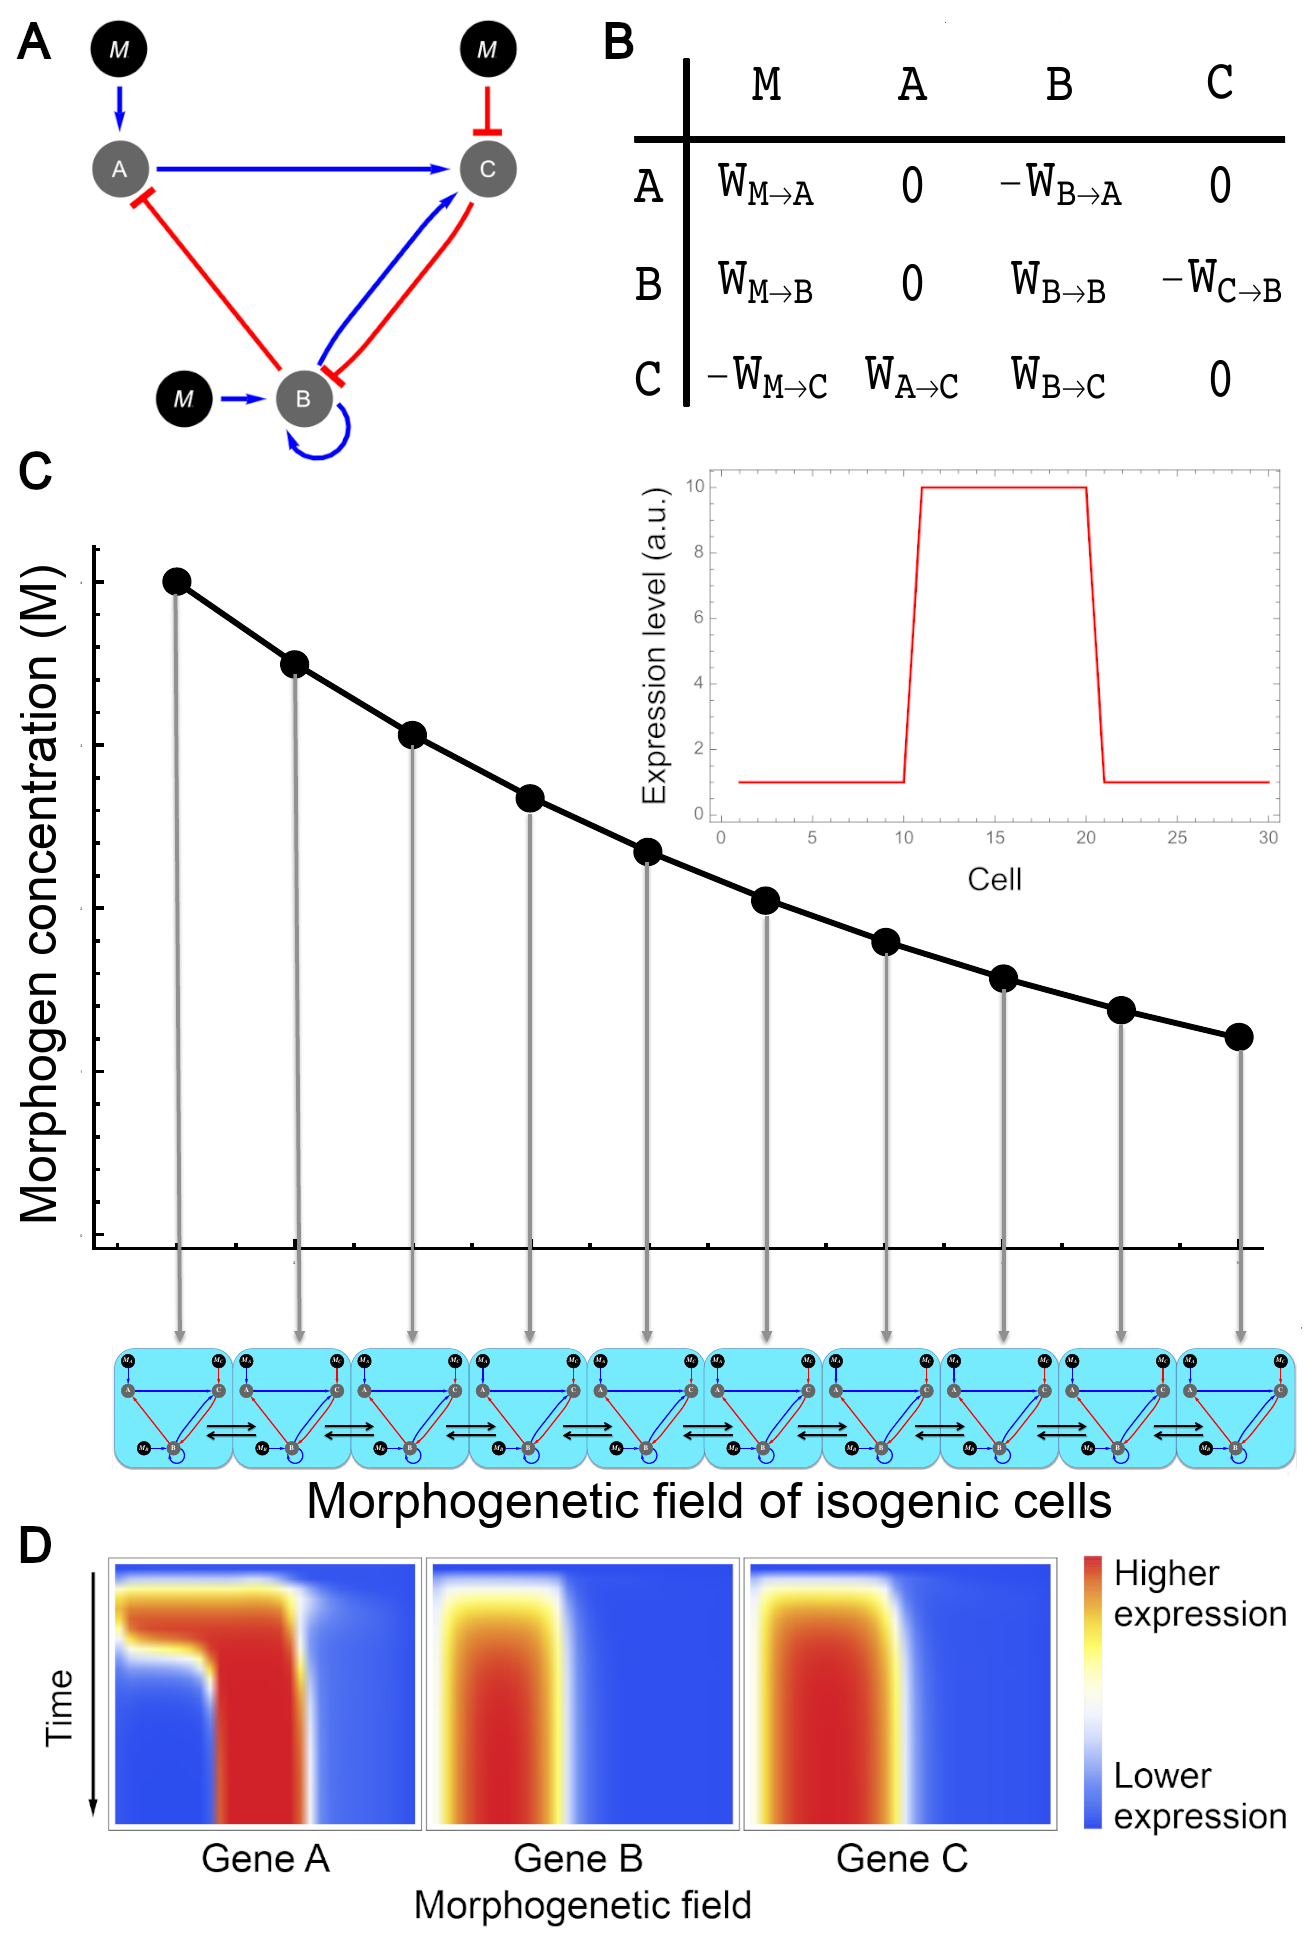
\includegraphics[width=\textwidth]{figures/metodos/Fig1}
    \caption{\bf Modelling of GRNs.}
    (A) GRN represented as a directed graph with activation (blue arrows) and
    inhibition (red arrows) interactions. Black circles
    tagged with a \textbf{M} represent the morphogen; \textbf{A}, \textbf{B} and
    \textbf{C} represent genes in the network.
    (B) The same GRN represented as an adjacency matrix in which positive values
    represent activation, negative ones represent inhibition and
    zeros represent no interaction.
    (C) Morphogenetic field. In our model the field was composed of a linear
    array of 30 isogenic cells and a morphogen gradient concentration described
    by an exponential decay function. Horizontal arrows between cells represent
    diffusion of gene products between adjacent cells. Optimal gene expression
    pattern is shown top right.
    (D) Heatmap of spatiotemporal expression profile of a GRN where blue
    colors represent lower expression and red colors represent higher
    expression.
 \label{fig:model}
\end{figure}

In our model the morphogen could interact with any of the three genes on the
GRN, but could not be affected by them. The morphogenetic field was defined by
an unidimensional array of 30 isogenic cells exposed to the morphogen
concentration gradient (Fig~\ref{fig:model}C). The initial concentration of
each gen product in all cells was set to 0.1 in all simulations.\\

\subsection*{Mathematical model}

Our model is a modification of the model used by Cotterell \& Sharpe~\cite{Cotterell2010}
and proposed by Reinitz et al.~\cite{Reinitz1995}. The
model is a dynamical system that describes the change in concentration of gene
product \emph{i} in time, as shown in Eq~\ref{ec:modelo-gral}.

 \begin{eqnarray}
  \frac{d[G]^i_n}{dt}
  = g(u^i) + D_i \cdot [ ([G]^i_{n-1}-[G]^i_n) +([G]^i_{n+1}-[G]^i_n)]-\delta_i
  \cdot [ G ]^i_n ,
  \label{ec:modelo-gral}
 \end{eqnarray}
\noindent
in which $[G]^{i}_{n}$ is the concentration of the i-th gene in the \emph{n}-th
cell ($[G]^{i}_{n} ≥ 0$), $g(u^i)$ is a function describing the relationship
between the interactions on the \emph{i}-th gene and its expression
Eq~(\ref{ec:input-func}) and described in more detail below. $D_i$ and
$\delta_i$ are the diffusion and the degradation rate of \emph{i}-th gene
product, respectively.\\

The input function is a sigmoid function described by Eq~\ref{ec:input-func}.
\begin{equation}
 g(u^i) = \frac{1}{1 + \exp(a - b \cdot u^i)},
 \label{ec:input-func}
\end{equation}
\noindent
in which $a$ is the sigmoid steepness, equal to 5; $a/b$ is the threshold value,
set to 1 for all simulations, and $u^i$ is the following equation:
\begin{equation}
 u^i = \sum_j w_{ij} \cdot [G]^j_n + w_{im} \cdot [M]_n.
 \label{ec:mat-sum}
\end{equation}

This equation sums the interactions acting upon the \emph{i}-th gene, being
$w_{ij}$ the interaction strength of the \emph{j}-th gene upon the \emph{i}-th
gene and $w_{im}$ the interaction strength of the morphogen upon the \emph{i}-th
gene. $[G]^j_n$ and $[M]_n$ are the concentrations of the \emph{j}-th gene
product and the morphogen in the \emph{n}-th cell.

\subsection*{Morphogen spatial distribution}

The morphogen concentration along the morphogenetic field is described by
Eq~\ref{ec:morph}.
\begin{equation}
 M = A_0 \cdot \exp(-c/h),
 \label{ec:morph}
\end{equation}
\noindent
were $A_0$ is the concentration of the morphogen in the position zero of the
morphogenetic field and was set to 1 in our experiments; $c$ is the cell index,
defined as the ratio between the \emph{n}-th cell from left to right and the
total number of cells, and $h$ is a decay parameter, whose value in our model
was set to 0.4.

The phenotype of a GRN was defined as the expression pattern of each gene along
the morphogenetic field after 500 time steps of integration of the dynamical
system. We chose that number of time steps because numerical experiments showed
that GRNs reached the steady state in approximately 300 steps (\nameref{S2_Fig}).

\subsection*{Optimal pattern definition}

The optimal pattern of gene expression defined by us, consisted in cells at the
sides of the field ($n<11$ and $n>20$) displaying expression levels lower than
10\% of the maximal level observed along the field of cells for the output gene,
and cells at the middle of the field ($n ∈ [11,20]$) displaying expression
levels greater than 90\% of the maximal level observed along the entire field
for the output gene (Fig~\ref{fig:model}C).

\subsection*{Genetic algorithm}

The genetic algorithm used to produce the set of gene regulatory networks (GRNs)
consisted in the following steps:

\begin{enumerate}
 \item{\bf Generate a random GRN.}

 \item{\bf Numerically solve the dynamical system for the GRN from t=0 until
 t=500.} We integrated the differential equation using the function NDSolve from
 Wolfram Mathematica 11 with the option “EquationSimplification” and the
 “Residual” simplification method.

 \item{\bf Evaluate fitness by comparing the GRN phenotype with the optimal
 phenotype (Fig~\ref{fig:model}C).} In order to compute the fitness
 function for each GRN we used three different filters. The first filter
 assesses whether the expression profile of the output node reaches a
 quasi-steady state:
 \begin{equation}
  S_{filter} = \left( \frac{1}{I \cdot N}\right) \sqrt{\sum_{i=1}^{I=3}
  \sum_{n=1}^{N=30} ([G]_n^i(t=500) - [G]^i_n(t=250))^2}.
 \end{equation}

 The expression profile was considered to have reached the steady state if
 $S_{filter} < 0.001$.\\

 The second filter measures the spatial heterogeneity in the field:
 \begin{equation}
  P_{filter} = \left( \frac{1}{I \cdot N} \right) \sqrt{ \sum_{i=3}^{I=3}
  \sum_{n=1}^{N=30} \left( [G]^i_n - \langle [G]^i_n \rangle \right)^2 },
 \end{equation}

 where $\langle [G]^i_n \rangle$ is the mean concentration of the \emph{i}-th
 gene along the field at $t=500$.\\

 The third filter relates the Manhattan Distance ($D_{obs}$) between an
 expression pattern and the optimal pattern with the maximum distance achievable
 ($D_{max}$):
 \begin{equation}
  \mathit{PF}_{eff} = 1 - \frac{D_{obs}}{D_{max}}.
 \end{equation}

 In this function, the expression profile of the output gene was normalized and
 discretized so that each expression value for each cell in the field was an
 integer ranging from 1 to 10.\\

 The filters mentioned above are integrated in the following functions that
 evaluates the  quality of a given phenotype:

 \begin{equation}
  Q_1(P_{filter}) = \left( \frac{ {P_{filter}}^{10} }{ {P_{filter}}^{10} +
  0.1^{10} } \right),
 \end{equation}
 \begin{equation}
  Q_2(S_{filter}) = \left( \frac{ 0.1^2 }{ {S_{filter}}^2 + 0.1^2 } \right).
 \end{equation}

 Finally, these quality functions were used to compute the fitness score with
 the following fitness function:
 \begin{equation}
  F = \mathit{PF_{eff}} \cdot Q_1(P_{filter}) \cdot Q_2(S_{filter}).
 \end{equation}

 \item{\bf Mutate GRN network parameters or gene product diffusion or
degradation rates randomly and evaluate fitness again.} If fitness of the
mutated GRN is greater than that of the previous GRN, save GRN and continue
mutating.

 \item {\bf Mutate GRNs randomly and evaluate fitness again.} Mutations
included changes in the  numerical values of degradation and diffusion
parameters and interaction strengths, and addition and removal of interactions
among genes and between the genes and the morphogen. If fitness of the mutated
GRN was greater or equal than that of the previous GRN, mutated GRN was saved
and the cycle continued from step 2. This cycle was repeated 5000000 times and
GRNs with a fitness greater or equal than 0.95 were saved into a file.

\end{enumerate}

Steps 1 to 5 were iterated 500 times, resulting in a set of 2061 GRNs with a
striped pattern of gene expression in at least one gene.

\subsection*{Classification of GRNs}

In order to group all the isomorphic networks in the set of 2061 GRNs we used a
classification algorithm that selected a random GRN, then it generated all
isomorphs of that GRN by performing permutations in rows and columns. The
algorithm then compared all six isomorphs with other GRN and classified the
topologies in the same group if they were isomorphic networks.

\subsection*{Neutral network}

The neutral network was obtained by generating all possible isomorphs of a
network topology and then calculating the minimal Hamming distance between these
isomorphs and other network topologies. The Hamming distance between two
topologies was calculated using the following equation:
\begin{equation}
 D_H(W^A, W^B) = \sum_{ij} \mid sgn(w_{ij}^A) - sgn(w^B_{ij}) \mid .
\end{equation}

We adopted the same definition of neighborhood as Cotterell \&
Sharpe~\cite{Cotterell2010}, in which two topologies were neighbors if the gain or
removal of any one interaction can transform one of the topologies into the
other.

\subsection*{Robustness analysis}

In order to evaluate the robustness of the different topologies to perturbations
in parameters of interactions between genes we took a GRN belonging to each one
of the network topologies and we modified each interaction independently by
increasing and decreasing its value by 20\%. For topologies with 3 or more
GRNs we chose the most similar to the mean configuration for that topology.\\

As a measure of the robustness of the topology we chose the proportion of times
in which a perturbation resulted in a GRN with a fitness greater or equal to
0.95. Additionally, we considered a topology to be robust if the previous
measure was greater or equal to 0.5.\\

As a measure of the robustness of subgraphs (see “Classification of topologies”)
we calculated the mean of the robustness measure of all the topologies
containing a particular subgraph.\\

\subsubsection*{Robustness of topology 9 to perturbations in non-network parameters}

In order to estimate the robustness of topology 9 to changes in parameters that
control morphogen gradient and changes in initial concentrations of gene
products, we generated 100 fitness values for each one of the 19 GRNs
belonging to topology 9; in each of these 100 assays we chose $A_0$, $h$ or
initial concentrations randomly from a Normal Distribution with $\mu = 1$ for
$A_0$, $\mu = 0.4$ for $h$ and $\mu = 1$ for initial concentrations and a
Coefficient of Variation of 30\% in each case.

\subsection*{Shannon entropy}

We calculated the Shannon entropy Eq~(\ref{ec:shannon}) of the network
topologies distribution in order to test if this distribution could be obtained
by chance with a probability greater than 0.05. In order to obtain a 95\%
confidence interval, we generated 30 samples of a set of 2061 random matrices
and calculated the Shannon entropy in bits for each sample and tested these data
for normality.
\begin{equation}
 H = -\sum p(x) \cdot \log_{2}p(x).
 \label{ec:shannon}
\end{equation}

\subsection*{Classification of GRNs phenotypes}

In order to classify each GRN by its spatiotemporal expression profile (its
dynamics of expression), we selected expression profiles of GRNs from time step
0 to time step 250 each 10 time steps, for a total of 26 expression profiles
over time. These spatiotemporal expression profiles were represented as tensors
$S \in \mathbb{R}^{3 \times 26 \times 30}$, in which each element ($s_{itn} \geq
0$) is the expression level of the \emph{i}-th gene at time $t$ in cell $n$.\\

Later we calculated the distance between all the pairs of tensors and we
performed a Neighbor Joining clustering using the package Scikit Bio 0.5.5 from
Python 3.

\subsection*{Classification of topologies}

In order to classify each topology by its subgraph composition, we first created
a matrix  $T = (t_{ij})$ with each row corresponding to a different topology
and 17 columns corresponding to subgraphs shown in \nameref{S4_Fig}.
Each element $t_{ij}$ of
the matrix was 1 if the \emph{j}-th subgraph was present in the \emph{i}-th
topology or 0 if the subgraph was not present.\\

With this matrix we then calculated a distance matrix in which each element
consisted in the Hamming distance between the row vectors in matrix $T$ between
each pair of topologies. We then performed a clustering of these topologies
using the Neighbor Joining method in the Scikit Bio package.

\subsection*{Complexity index and network descriptors}

As a measure of network complexity, we used the complexity index based on
Shannon entropy proposed by Bonchev \& Rovray~\cite{D.2005}. We calculated this
index using the following equation:
\begin{equation}
 I_{vd} = \sum_{i=1}^V a_i \cdot \log_{2} a_i,
\end{equation}
\noindent
being $a_i$ the degree of \emph{i}-th node and $V$ the number of nodes in the
network. The network descriptors were calculated using built-in functions from
Wolfram Mathematica software.\\

We performed a Pearson’s chi-square goodness of fit test for the node degree
distribution using Wolfram Mathematica.

% For placing video, \nameref{S1_Video} vel sagittis arcu lobortis.

% Place figure captions after the first paragraph in which they are cited.
% \begin{figure}[!h]
% \caption{{\bf Bold the figure title.}
% Figure caption text here, please use this space for the figure panel descriptions instead of using subfigure commands. A: Lorem ipsum dolor sit amet. B: Consectetur adipiscing elit.}
% \label{fig1}
% \end{figure}

% Results and Discussion can be combined.
\section*{Results}

The classification of GRNs showed that our initial set of 2061 GRNs can be
grouped in a number of 714 distinct network topologies, each one of them
containing a different number of GRNs (Fig~\ref{fig:distopol}). This abundances
distribution was not produced by chance (Shannon entropy = 8.52963, 95\%
confidence interval = [10.8915, 10.9275]), and instead it displays some level
of structure, indicating the existence of network motifs.

\begin{figure}[!h]
 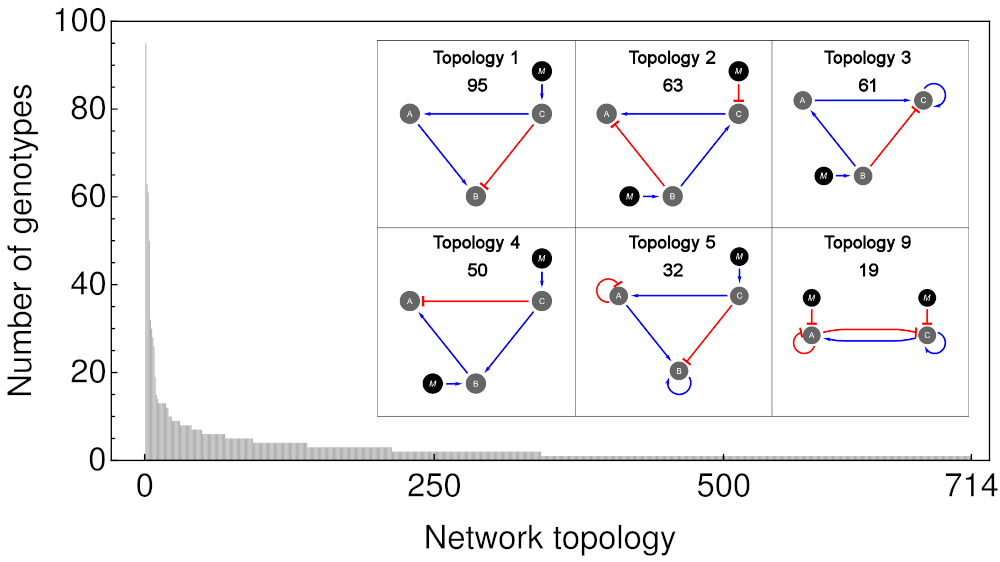
\includegraphics[width=\textwidth]{figures/results/Fig2}
 \caption{\bf Distribution of abundances of network topologies.}
 Some of the most frequent network topologies shown in the grid
 contain the I3-FFL network motif (shown on the left). In this network
 motif the gene B is activated in an indirect way by the morphogen through
 the activation of A (positive interactions), and at the same time, it
 is inactivated in a direct way by the morphogen (negative interaction).
 Topologies are numbered in order of decreasing abundance, being the
 Topology 1 the most abundant with a number of 95 genotypes. The number of
 genotypes belonging to each network topology is presented below
 topology number.
 Note that network topology number 9 produces the striped phenotype using a
 two-node GRN.
 \label{fig:distopol}
\end{figure}

The most abundant network topologies are shown in Fig~\ref{fig:distopol}.
Interestingly, among the 15 most abundant network topologies, eleven of them
presented the Incoherent type 3 Feed-Forward Loop (I3-FFL) network motif. In
addition, we found that topology number 9 could produce the striped phenotype
with only two nodes.

The neutral network (a metagraph in which each node is a network topology)
shows that most of the network topologies are grouped into a connected graph.
This graph is composed of 639 nodes that are accessible by one mutational step.
The 15 most abundant network topologies, with the exception of
number 10, are part of this graph (Fig~\ref{fig:neutral-network}). We also
found nodes inside the neutral network that had more connections between them
than with other nodes, generating clusters of nodes, interestingly in
almost every cluster is present one or more of the 15 most abundant network
topologies. In addition, we found that the first eight most abundant network
topologies were located in the largest cluster.

\begin{figure}[!h]
 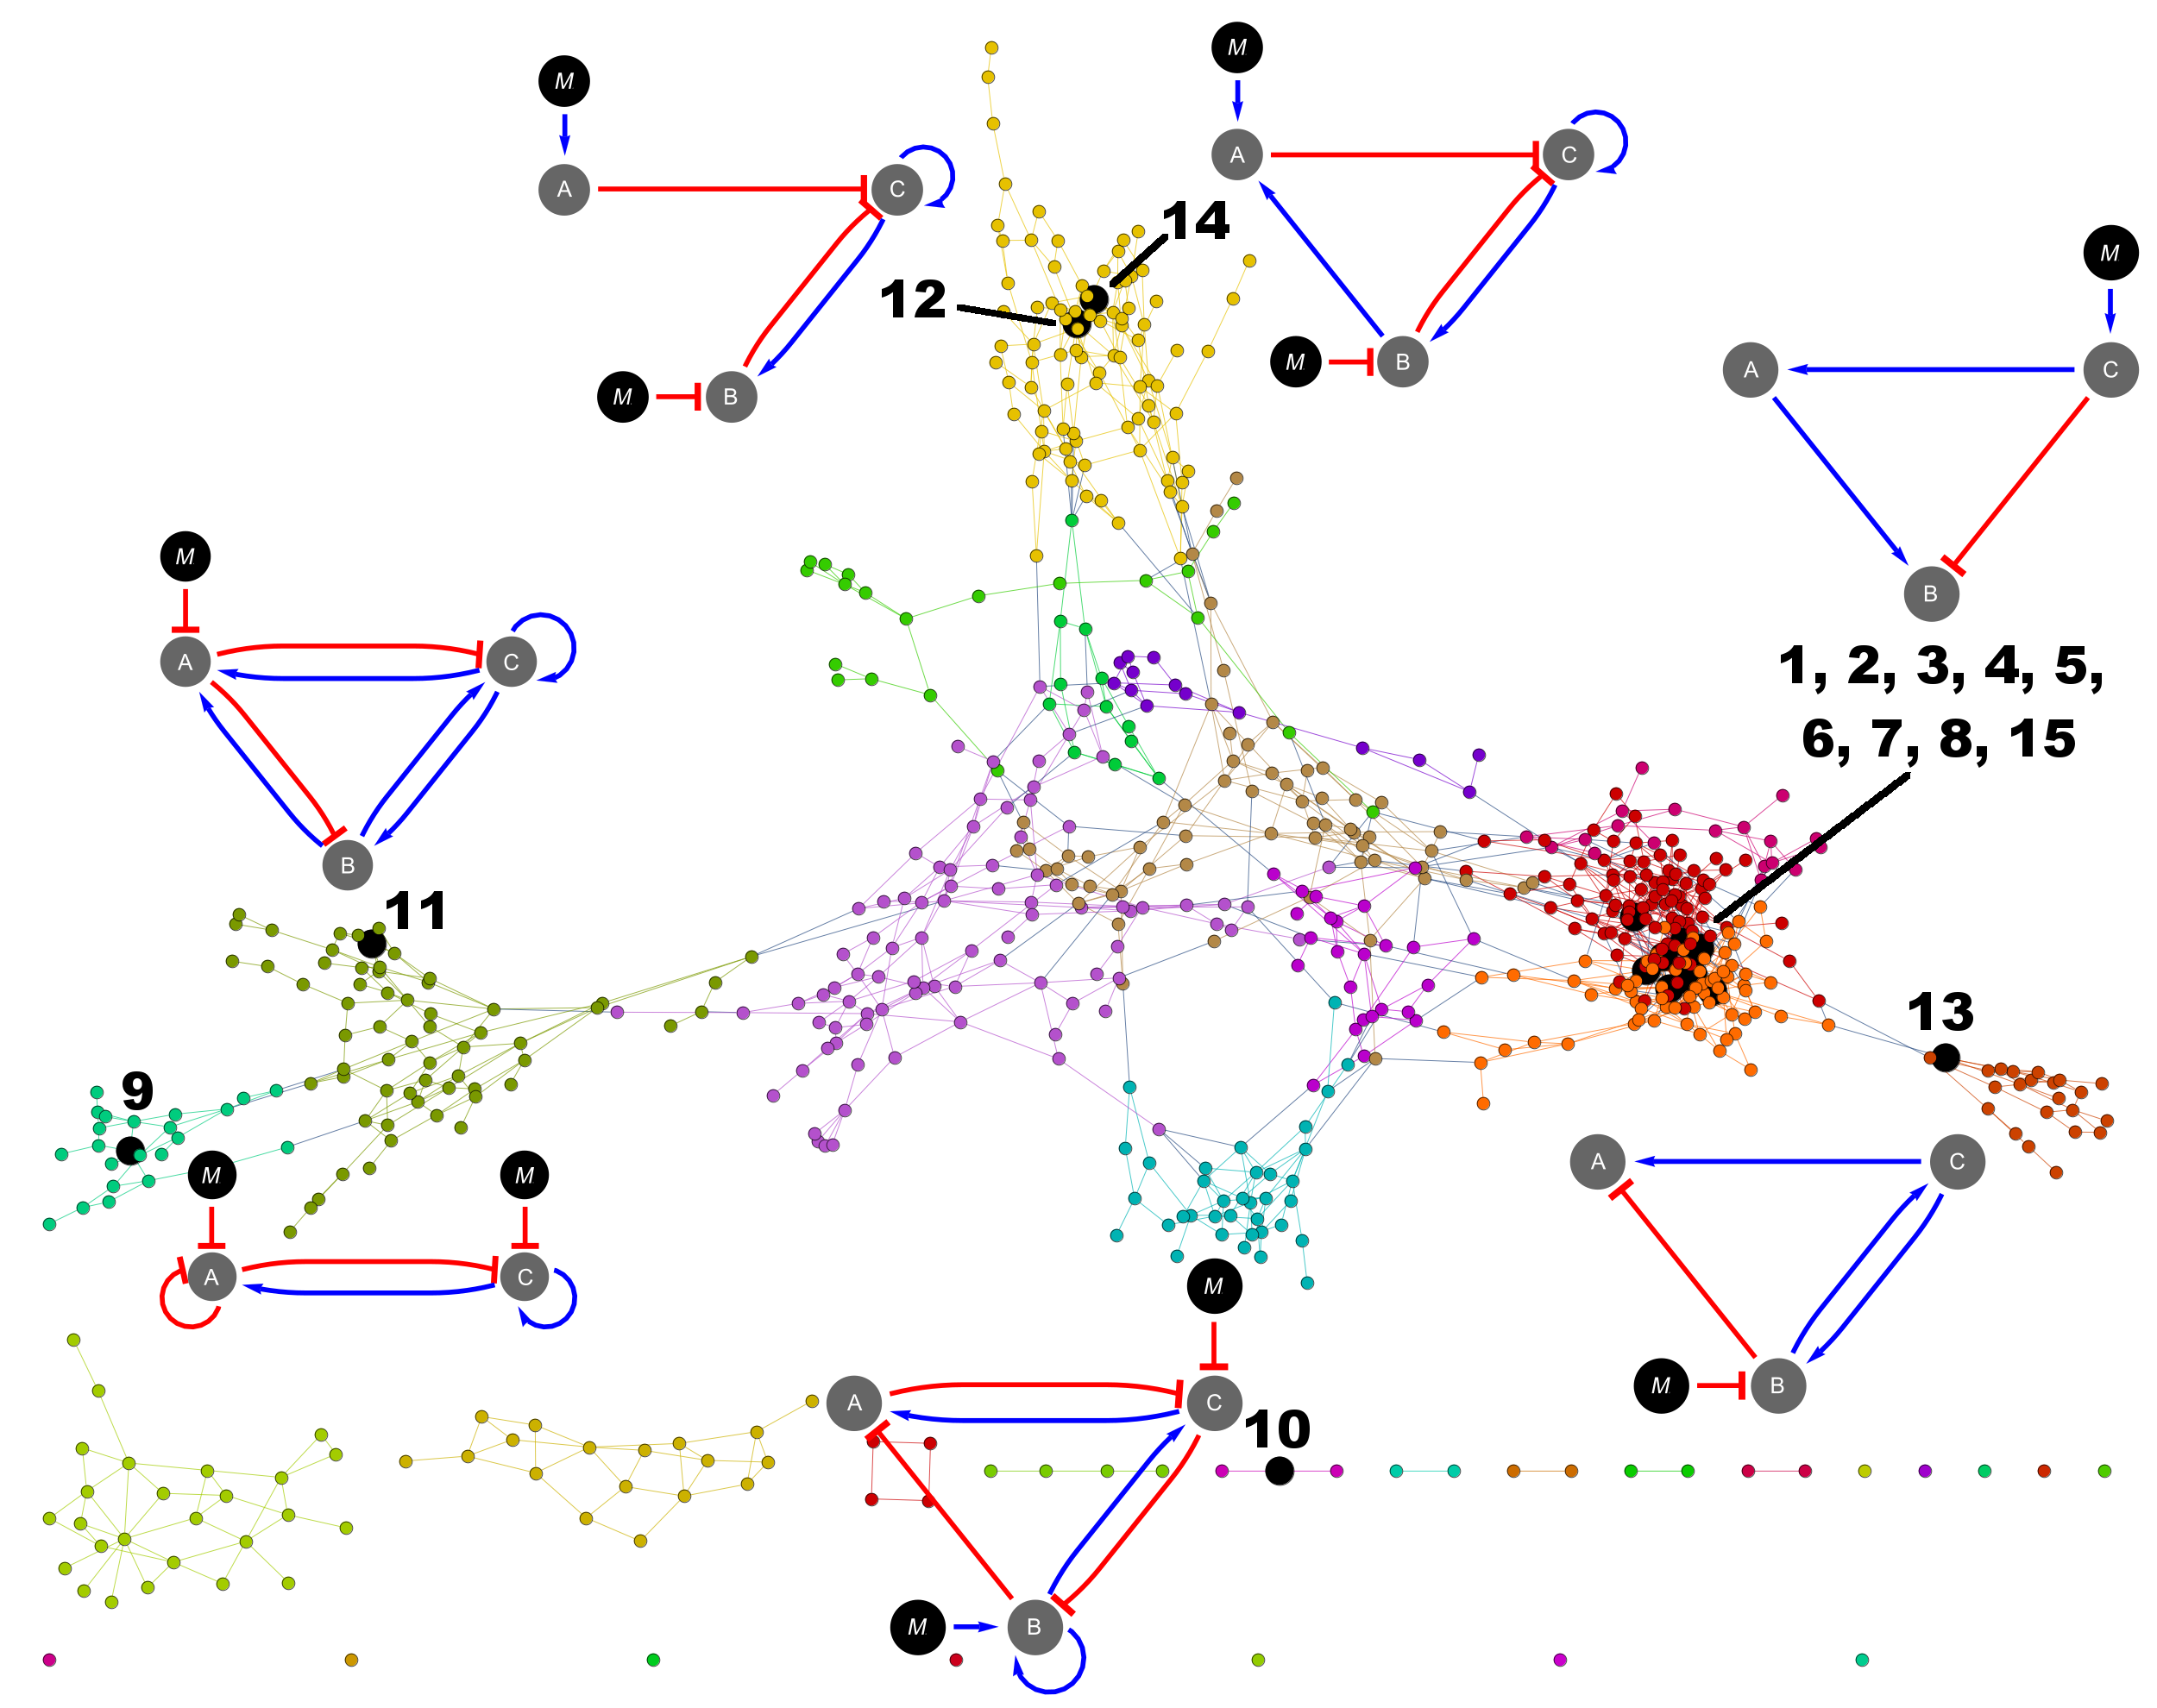
\includegraphics[width=\textwidth]{figures/results/Fig3}
 \caption{\bf Neutral network.}
 This graph shows network topologies connected by one mutational step, where
 each node represents a single topology. Black nodes represent the most
 abundant topologies. All nodes with the same
 color belong to a cluster of nodes more connected between them than with other
 nodes in the graph. The most abundant topologies are represented as
 directed graphs in the same way as in Fig~\ref{fig:model}A, except for
 the topologies 1 to 8 and 15 (orange and red clusters), in which only
 topology 1 is depicted.
 \label{fig:neutral-network}
\end{figure}

The degree distribution of this network seems to follow a Poisson distribution
(Pearson’s $\chi^2 = 12.8902$, $\text{p-value} = 0.115684$) characteristic of a
Erdös-Rényi network with many nodes and edges~\cite{Erdos1959}. This kind of
network presents a great
number of nodes with low degree and a few nodes with high degree
(Fig~\ref{fig:deg-dist}A). Nodes corresponding to topologies number one and
three showed the highest degree ($deg(1) = deg (3) = 14$). Curiously, nodes with
higher degree resulted to be also those network topologies with higher abundance
(Fig~\ref{fig:deg-dist}B). This relationship between abundance and node degree
was corroborated by the Spearman's rank correlation coefficient
($r_S = 0.353752$, $p = 6.2933\times10^{-23} $).

\begin{figure}[!h]
 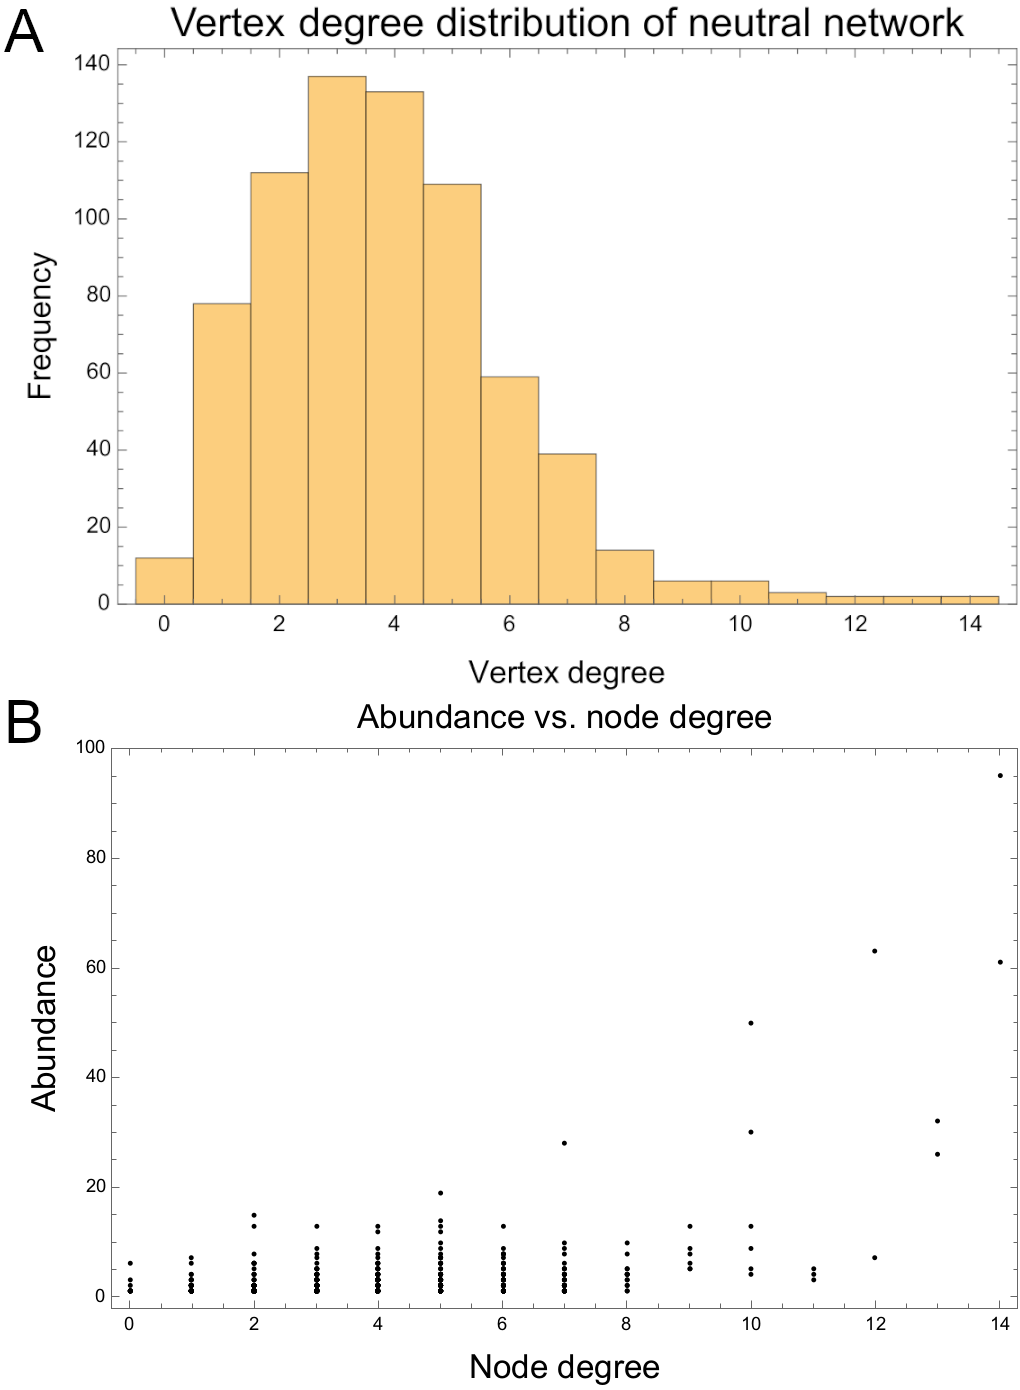
\includegraphics[width=\textwidth]{figures/results/Fig4}
 \caption{\bf Node degree in the neutral network.}
 (A) Histogram of vertex degree distribution in the neutral network.
 (B) Scatter plot of Topology abundance vs. Node degree in the neutral
 network.
 \label{fig:deg-dist}
\end{figure}

We wanted to know if connecting topologies separated by two mutational steps
would produce a connected graph, for that reason we generated another neutral
network joining neighbors at two mutational steps and we found that only
topology number 420 remained unconnected from the rest of topologies in the
graph (Fig~\ref{fig:2neut-net}).

\begin{figure}
 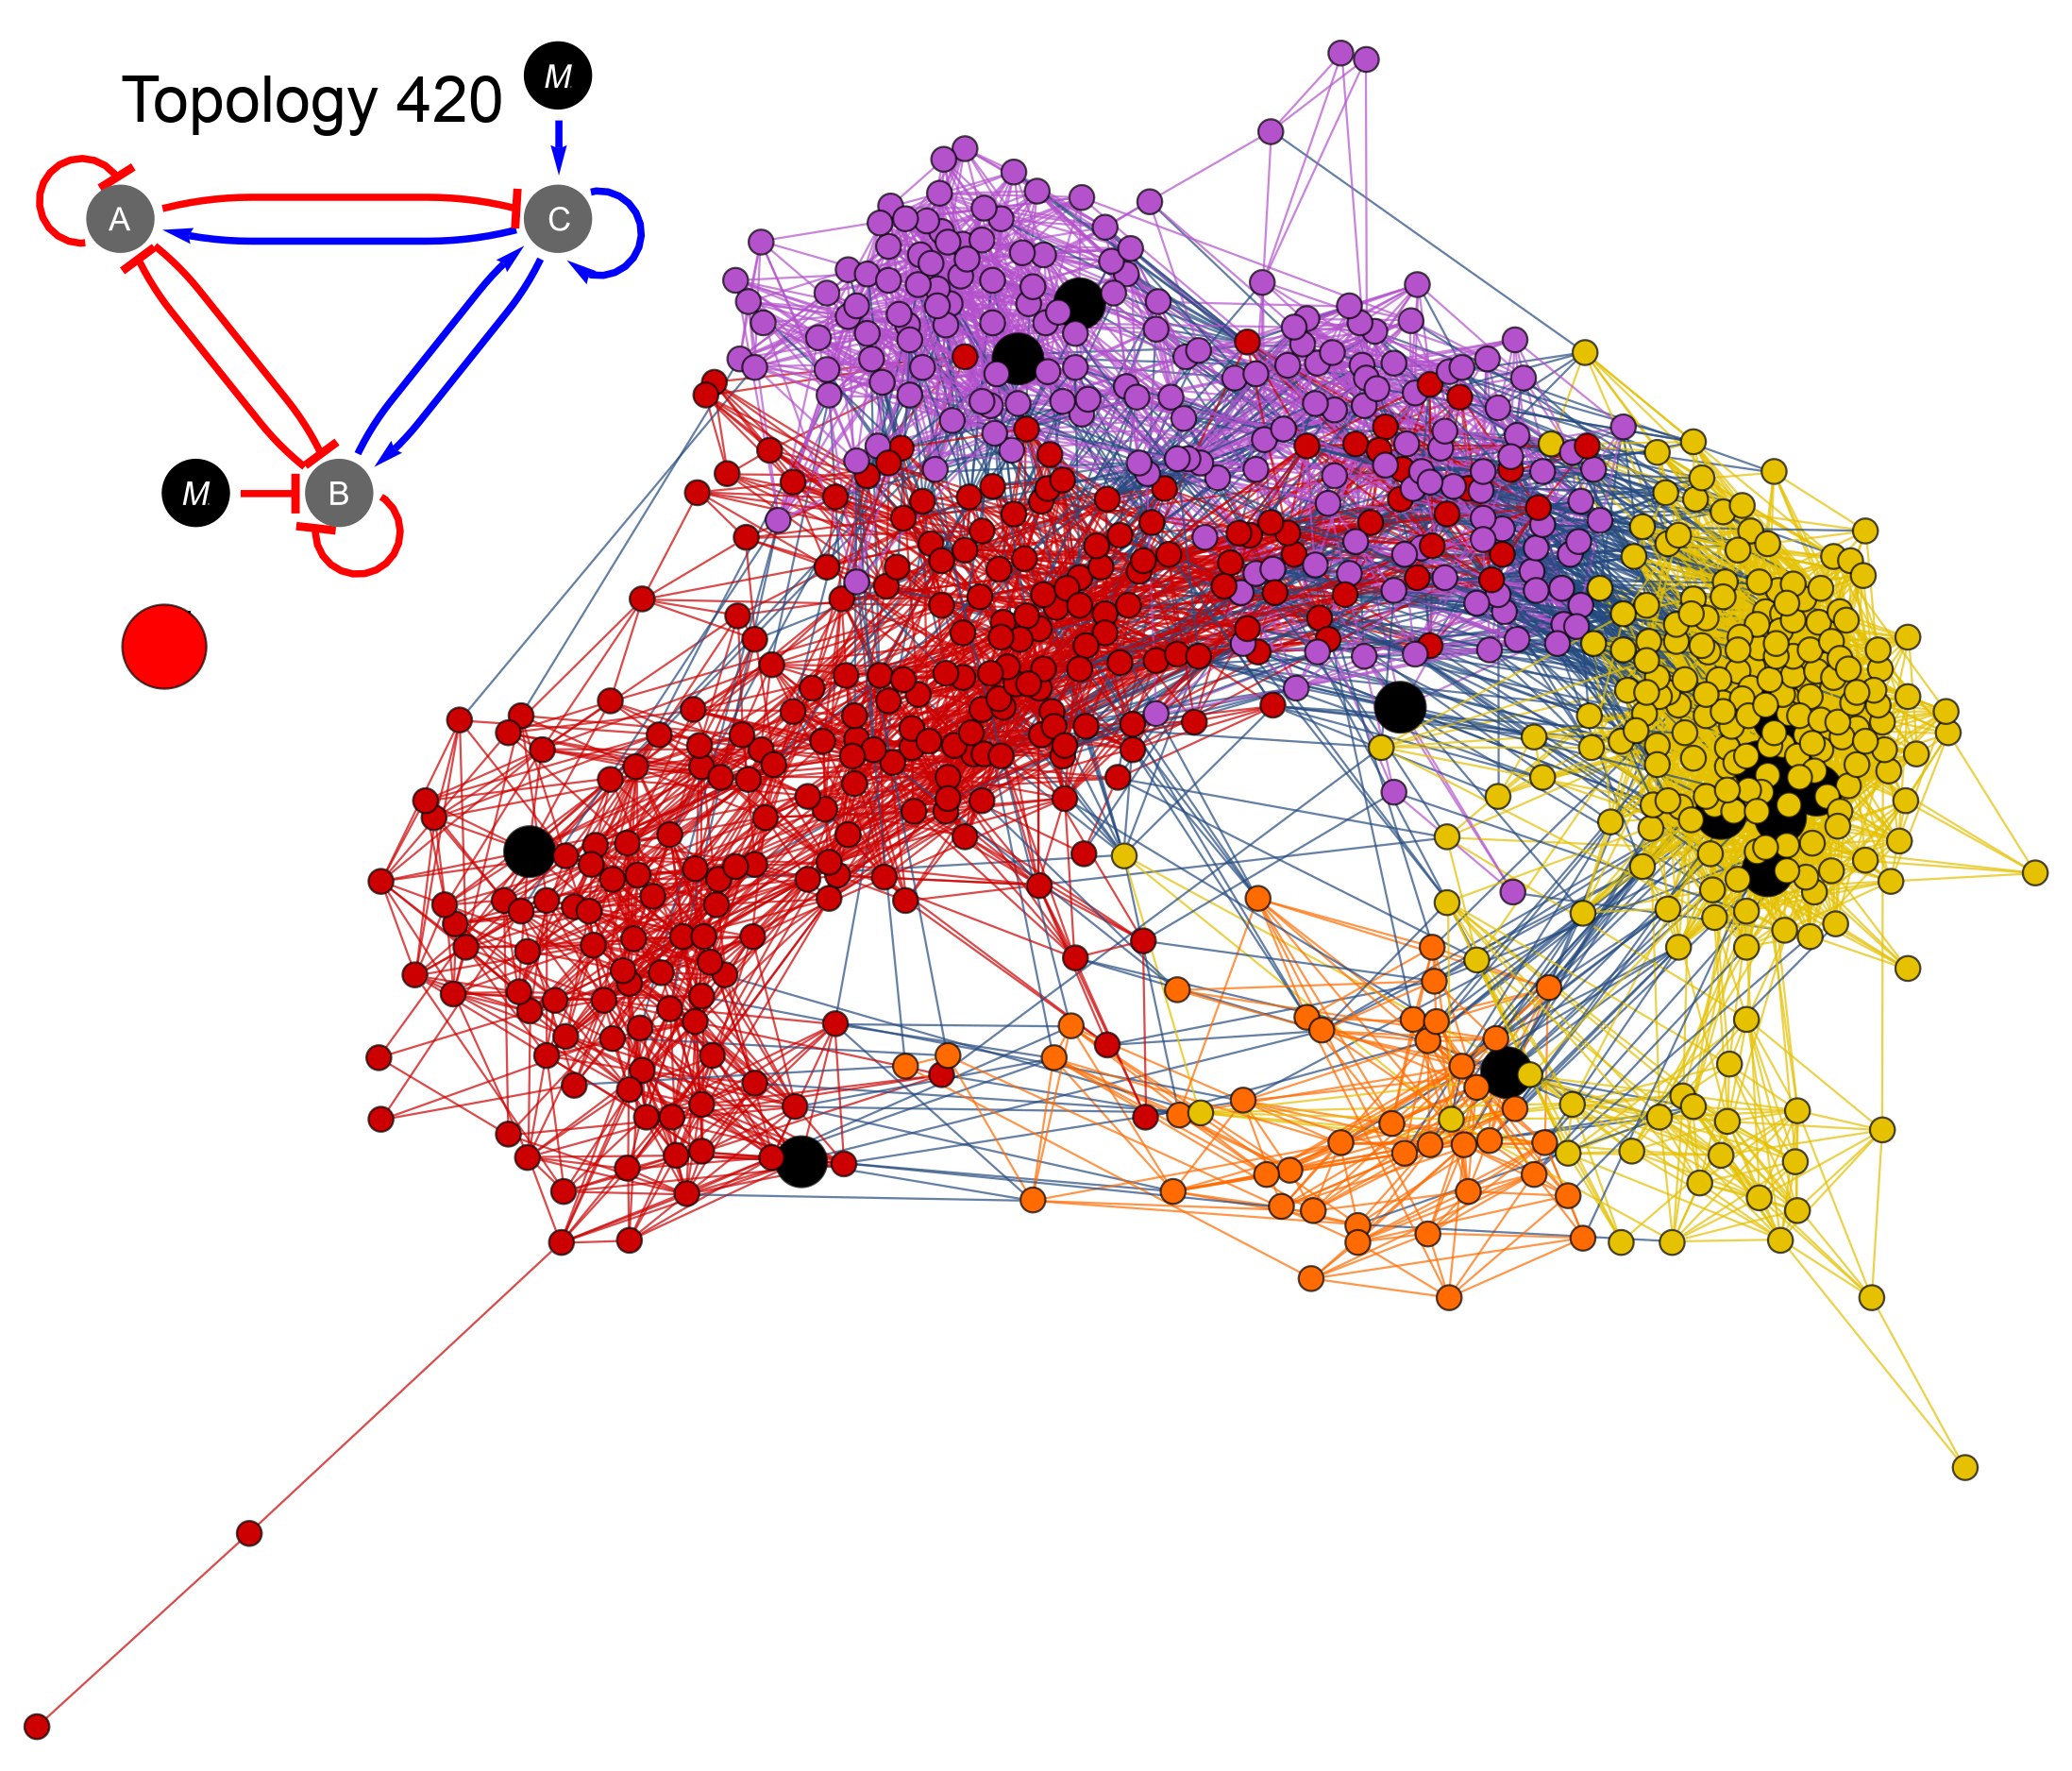
\includegraphics[width=\textwidth]{figures/results/Fig5}
 \caption{\bf Network of topologies separated by two mutational steps.}
 The network shows that almost all the topologies are connected by two or less
 mutational steps. Big red circle represents topology 420 that remains
 unconnected from the main graph. Big black circles correspond to the 15
 most abundant topologies described in Fig~\ref{fig:neutral-network}.
 Different colors in the graph represent different clusters of topologies.
 \label{fig:2neut-net}
\end{figure}

Besides topological robustness, we wanted to know if network topologies were
robust to perturbations in the values of the parameters. After performing the
perturbations to a GRN from each topology, we plotted the abundance of the
topology vs. its robustness. We did not find a significant correlation between
these two variables ($r_S = −0.0389724$, $\text{p-value} = 0.298475$)
(Fig~\ref{fig:ab-rob}A). However, when we grouped those topologies containing
the same subgraph and calculated their mean robustness, we found that between
the most robust subgraphs is the ``Bistable'' motif reported by Cotterell \&
Sharpe~\cite{Cotterell2010}, the I3-FFL and the ``Overlapping domains'' motif
(which is a variation of the I3-FFL) also reported by Cotterell \& Sharpe
(see \nameref{S4_Fig} and \nameref{S1_Table}).

\begin{figure}[!h]
 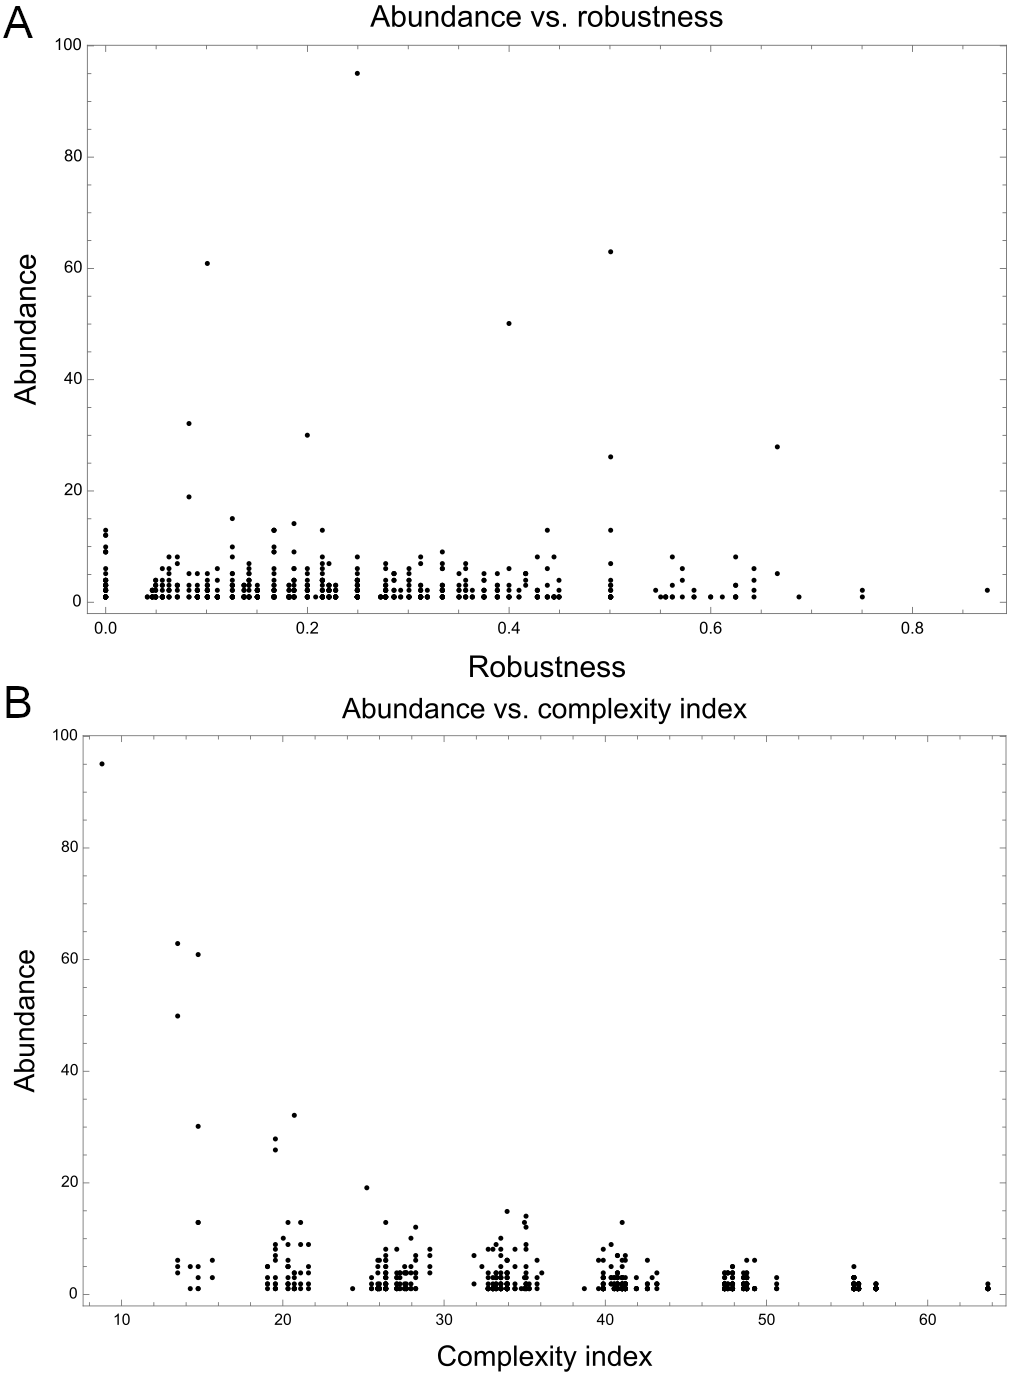
\includegraphics[width=\textwidth]{figures/results/Fig6}
 \caption{\bf Relationship between Abundance and robustness and complexity
 index.} (A) Abundance vs. Robustness. The robustness of each topology was
 calculated as the ratio of perturbations in which the fitness was greater or
 equal to 0.95 with respect to the total of perturbations performed.
 (B) Abundance vs. Complexity index. Each point in the plot represents one of
 the 714 network topologies. More complex topologies tend to be less abundant
 than simple topologies
 ($r_S = -0.316653$, $\text{p-value} = 2.25161\times10^{-18}$).
 \label{fig:ab-rob}
\end{figure}

The average vertex degree indicates that in general all the network topologies
display high robustness and that they could resist an average of approximately 4
topological mutations without losing their fitness. Additionally, the average
path length indicates that the evolutionary landscape is easily accessible for
most network topologies (Table~\ref{table1}).

\begin{table}[!ht]
% \begin{adjustwidth}{-2.25in}{0in} % Comment out/remove adjustwidth environment if table fits in text column.
 \centering
 \caption{{\bf Network descriptors of neutral network of topologies.}}
 \begin{tabular}{|l|l|}
 \hline
 {\bf Network descriptor} & {\bf Value}\\ \thickhline
 Average vertex degree  & 3.85714 \\ \hline
 Clustering coefficient~\cite{Watts1998} & 0.117097 \\ \hline
 Average path length    & 7.25261       \\ \hline
 Graph connectedness    & 0.00540974    \\ \hline
 Graph diameter*        & 25            \\ \hline
 Average path length*   & 9.0499        \\ \hline
 \end{tabular}
 \begin{flushleft} *These descriptors were calculated for the main connected
 subgraph of the network.
 \end{flushleft}
 \label{table1}
% \end{adjustwidth}
 \end{table}

The average complexity index of network topologies was 39.2435 ($\pm 11.6768$)
and was found to be negatively correlated with the abundance ($r_S = -0.316653$,
$\text{p-value} = 2.25161\times10^{-18}$) (Fig~\ref{fig:ab-rob}B).

Hierarchical clustering of spatiotemporal expression profiles showed that GRNs
with topologies that seemed to be very different have indeed very similar
expression dynamics. We expected to find GRNs with the same topology to group
together but instead we found GRNs with different topologies grouped as close
neighbors (Fig~\ref{fig:clustering}A). More interestingly, some GRNs displaying
very abundant network topologies were grouped together with GRNs displaying
very infrequent network topologies.

\begin{figure}[!h]
 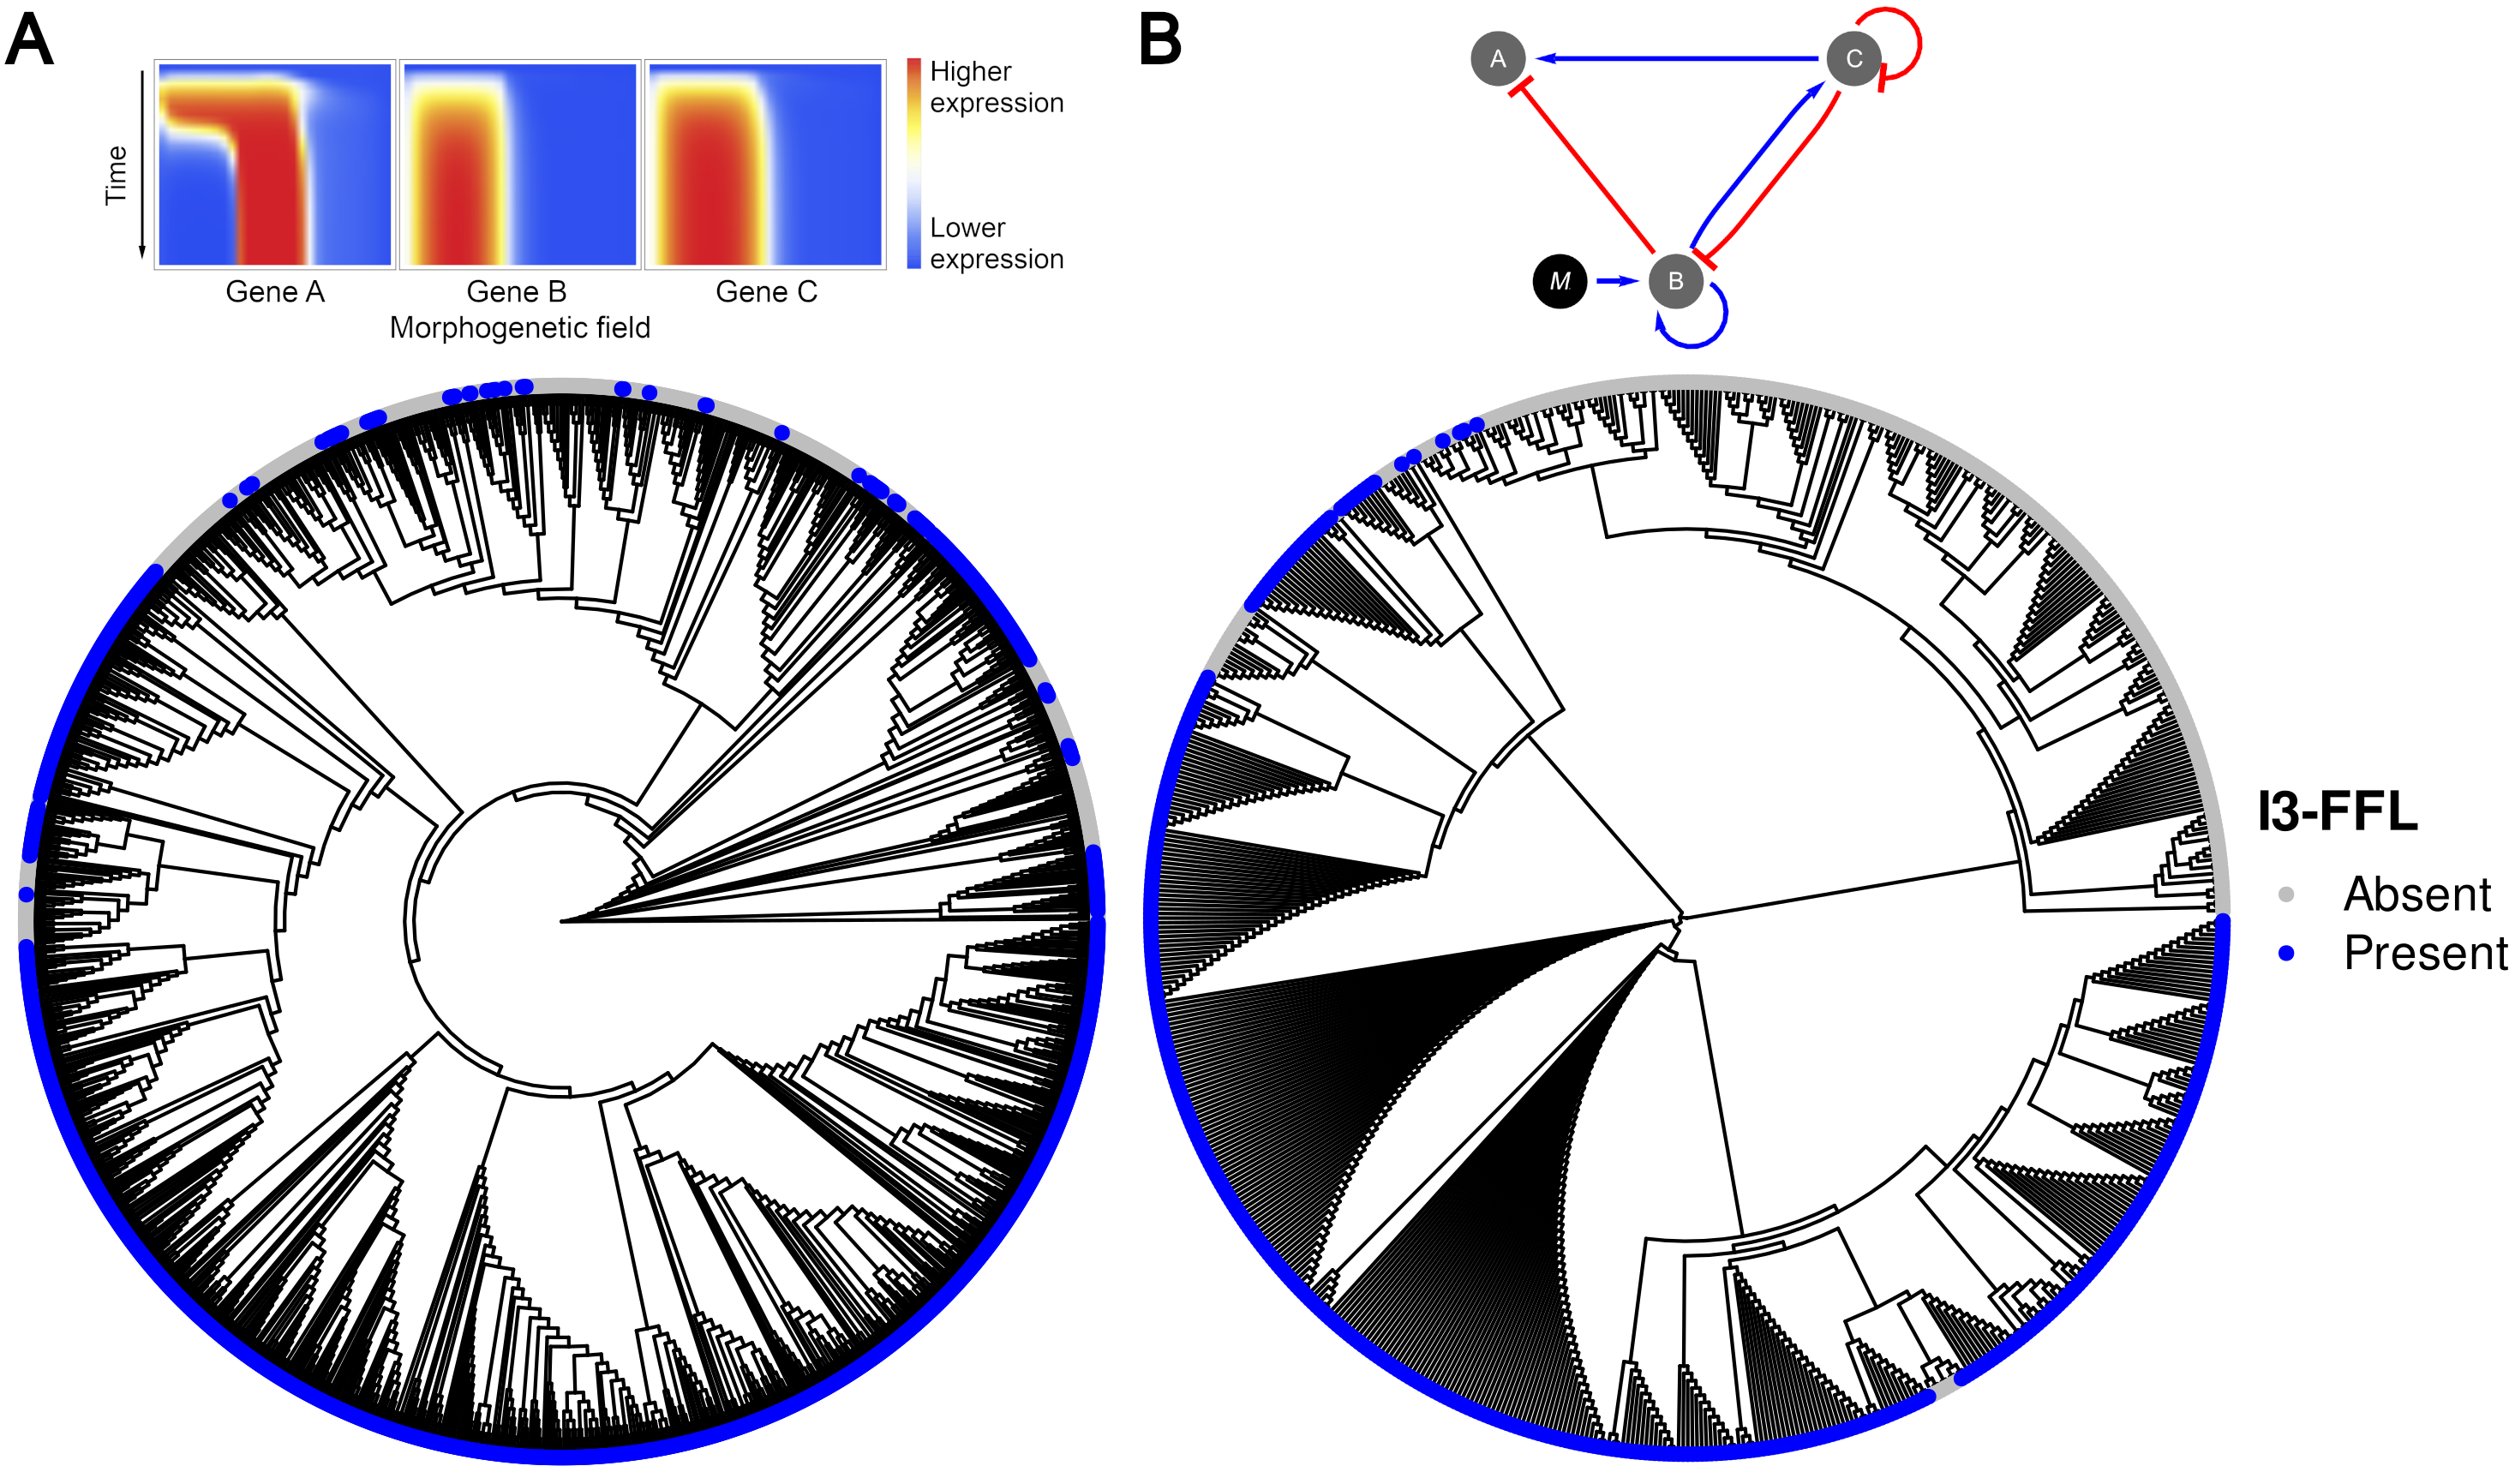
\includegraphics[width=\textwidth]{figures/results/Fig7}
 \caption{\bf Clustering of expression profiles and topologies.}
 (A) Clustering of spatiotemporal expression profiles obtained by
 neighbor joining. (B) Clustering of network topologies. Blue circles
 correspond to topologies that contain the I3-FFL network motif.
 \label{fig:clustering}
\end{figure}

Clustering of topologies revealed that there are six main groups of topologies
in our set of 2061 GRNs (Fig~\ref{fig:clustering}B).

Among the new network topologies we report here, perhaps the most interesting
is the topology number 9, which is able to express the striped gene expression
pattern with only two genes and indeed expresses this pattern in both genes
(Fig~\ref{fig:topol9}).

\begin{figure}[!h]
 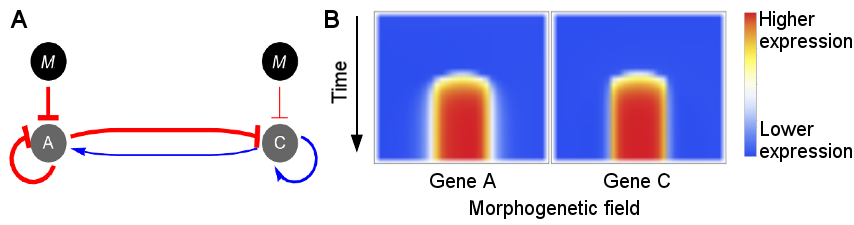
\includegraphics[width=\textwidth]{figures/results/Fig8}
 \caption{\bf Expression dynamics of topology 9.}
 (A) Network topology number 9. Although this topology consists only of two
 genes, it display a striped pattern of gene expression for both of them as
 can be observed in (B). (B) Spatiotemporal expression profile of a GRN
 with topology 9. Gene \textbf{B} is not shown as it was lost in this topology
 in the evolutionary process simulated by the genetic algorithm.
 \label{fig:topol9}
\end{figure}

Although the topology 9 consists of only two genes, its mechanism of expression
is dynamically more complex than that of other topologies such as the simple
I3-FFL. Initially the expression pattern of the gene A is uniform in the
morphogenetic field, but later it is shaped by the morphogen gradient in such a
way that two important events occur, in first place the overall expression
level of the gene A is decreased by the inhibition of the morphogen, releasing
gene C from its repression by gene A; in second place, it appears a
non-homogeneous spatial distribution in which gene A is expressed at higher
levels in the cells at the rightmost part of the morphogenetic field.\\

These two events conduce to the repression of the gene C by the gene A in the
rightmost part of the morphogenetic field and by the morphogen in the leftmost
part of the morphogenetic field, thus generating a slightly higher level of
expression of gene C in the center of the field. Because gene C activates its
own expression, a band of expression begins to form. This band of expression
then begins to activate the gene A also in the center of the field
(\nameref{S1_Fig}).
% (Fig~\ref{fig:topol9-dyn}).

% \begin{figure}[!h]
%  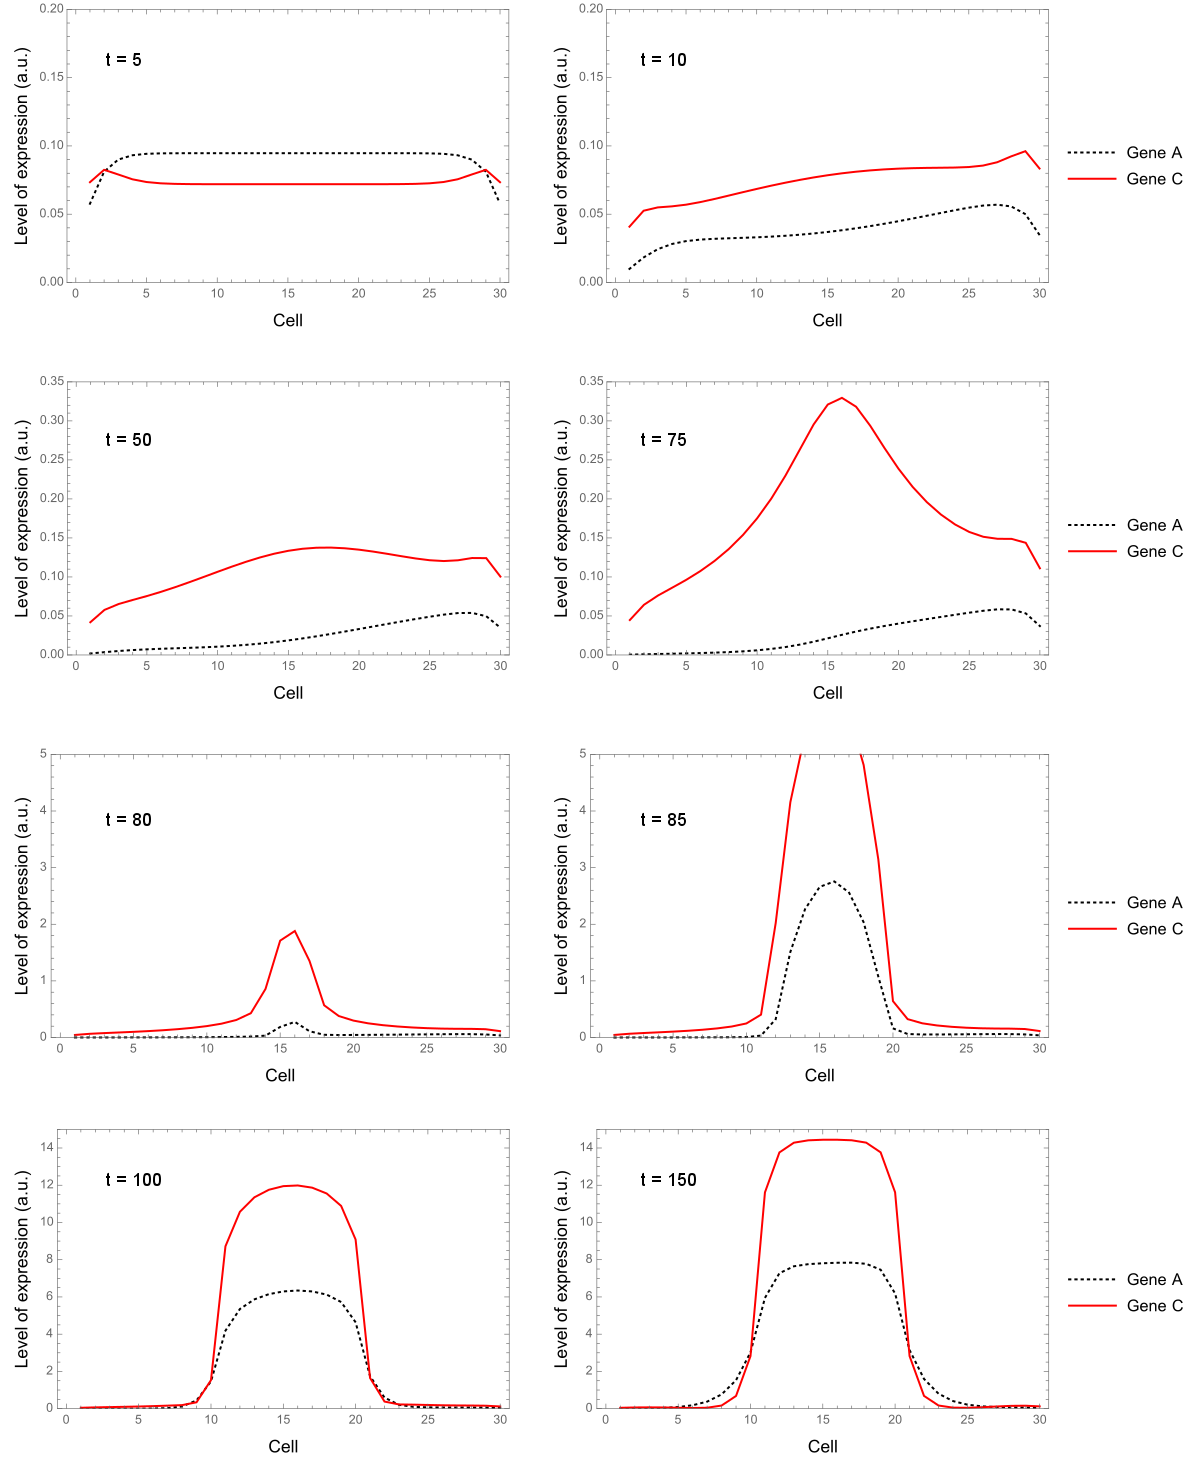
\includegraphics[width=\textwidth]{figures/results/topol-9-dynamics}
%  \caption{\bf Dynamics of expression in topology number 9.}
%  \label{fig:topol9-dyn}
% \end{figure}

In this way two bands of expression that depend on each other are formed. The
high level of gene C in the middle of the field counteract its inhibition by
gene A, while at the ends of the bands the inhibition of gene A on gene C
overcomes the self-activation of gene C, preventing the expression of the
latter to extend out of the middle of the field. In turn, the band of
expression of gene A can only exist in the middle of the field because its
expression depends on gene C.

This is a complex mechanism described by the first time in this study, and it
would be interesting to study its feasibility and possible implementation in
synthetic gene regulatory networks.

\section*{Discussion}

This study can help us to understand the mechanisms by which the GRNs work in
nature as modules that make part of genomes, and it also can provide guidance
in the construction of new synthetic GRNs in the field of synthetic biology.

We found the presence of network motifs in the set of GRNs produced by the
genetic algorithm. However, we also found a great diversity of network
topologies that could produce a striped gene expression pattern.\\

Robustness is an important feature of patterning mediated by morphogens, and
the GRNs involved can be selected in an evolutionary process not only by its final
steady state but also by its ability to buffer noise~\cite{lo_robust_2015, exelby_2021}.
In our study, the most abundant topologies were
found to be part of highly connected clusters in the neutral network, and this fact
indicates that these topologies are both robust to quantitative changes in the
strength of interactions and diffusion and degradation parameters as well as to
qualitative changes in the topology itself. As robustness and evolvability are
not mutually exclusive properties~\cite{wagner_robustness_2008}, it is likely
that these topologies are also evolvable.

Other studies have shown that Incoherent Feed Forward Loops are able to form
spatial stripes of gene expression~\cite{ishihara_cross_2005}. In particular,
we found that the I3-FFL is one of the network motifs that appears more
frequently in these GRNs, as has also been reported by Cotterell \&
Sharpe~\cite{Cotterell2010}, and has been found in transcriptional networks involved
in cell fate definition~\cite{Li2019}. Moreover, our results indicate that this
is a robust motif that can be useful for construction of synthetic gene
regulatory networks that are exposed to stochastic fluctuations in the
environment and mutations.

However, as our model was less stringent and allowed the morphogen input to
interact with any gene, we found a larger number of possible topologies with the
same striped phenotype. For example, in a single input model the I4-FFL could
not produce a stripe of gene expression~\cite{munteanu_2014}, whereas in our
experimental setup 20.17\% of the topologies presented this motif as a
subgraph~(\nameref{S1_Table}).

Although it has been experimentally demonstrated that the Incoherent Feed
Forward Loop type 2 (I2-FFL) is able to generate a striped gene expression
pattern,~\cite{Schaerli2014, Basu2005}, in our study this motif was present in
only 10.92\% of the topologies. This fact may be because genetic algorithms
can not always find global minima but local minima or its surroundings, however,
it is also possible that the I2-FFL motif is not as robust as other motifs and
therefore be less represented.

We also found topologies with a similar topology to that of the “opposing
gradients” reported by Schaerli et al.~\cite{Schaerli2018,Schaerli2014}.
Although the “opposing gradients” mechanism requires the constitutive expression
of two of the genes in the GRN, and our model does not take constitutive
expression into account, we realized that the GRNs that presented the “opposing
gradients” topology, had also commonly positive auto-regulation interactions on
these two nodes, supplying in this way the lack of constitutive
expression as found in previous studies~\cite{munteanu_2014}.

The correlation between the complexity index of a topology and its abundance
indicates that networks with simpler designs are more robust to changes in
interaction parameters and that more complex networks are less robusts. For
example, topology number 420 (Fig~\ref{fig:2neut-net}), which
presents high complexity, was one of the
topologies with lower abundance and was disconnected from all other topologies
in the two-step neighbors in the neutral network.

The cladogram of spatiotemporal expression profiles shows that the genetic
algorithm selected similar expression mechanisms that can be produced by very
different topologies.

Although GRNs that produce a band of gene expression with only two nodes have
been described (e.g. the I-zero motif,~\cite{Schaerli2014}) this is to our
knowledge the first time a GRN with a topology such as that of topology nine
(Fig \ref{fig:topol9})
and its expression mechanism are reported, increasing our knowledge of the
genotype-phenotype map in this kind of system, and it would be very interesting
to confirm experimentally the ability of this topology to generate the described
pattern and it would be interesting to study its feasibility and possible
implementation in synthetic gene regulatory networks.

%\section*{Conclusion}

%Aliquam tincidunt, ex in facilisis elementum, libero lectus luctus est, non vulputate nisl augue at dolor. For more information, see \nameref{S1_Appendix}.

\section*{Supporting information}

% Include only the SI item label in the paragraph heading. Use the \nameref{label} command to cite SI items in the text.

\paragraph*{S1 Fig.}
\label{S1_Fig}
{\bf Dynamics of expression of topology number 9.}
The dynamics of expression is shown from $t = 5$ to $t = 150$. The red line
represents the expression level of the gene C along the morphogenetic field,
whereas the dotted line represents the expression level of gene A. The
striped pattern of gene expression can be seen for both genes since $t = 80$.

\paragraph*{S2 Fig.}
\label{S2_Fig}
{\bf Most GRNs reach the steady state before 250 time steps.}
(A) Gene regulatory network displaying the topology number 33. (B) Spatiotemporal
expression profile of the gene regulatory network shown in (A).

\paragraph*{S3 Fig.}
\label{S3_Fig}
{\bf Bridge topologies in the neutral network.}
``Bridge topologies'' are those topologies that connect two clusters in the neutral
network (Fig~\ref{fig:neutral-network}), and as such can be interpreted as
intermediary steps in the evolution from a cluster of related topologies into
another cluster. For example the topology 441 could be an initial step to reach the
topology 9, as in this topology nodes B and C are not connected.

\paragraph*{S4 Fig.}
\label{S4_Fig}
{\bf Relevant subgraphs present in the set of GRNs.}
These are subgraphs that have been reported in previous studies as networks
involved in morphogenesis and development~\cite{Cotterell2010, Schaerli2014,
Schaerli2018}. These were used to calculate the subgraph profile and the results
reported in \nameref{S1_Table}.

\paragraph*{S1 Table.}
\label{S1_Table}
{\bf Proportion of relevant subgraphs in the set of GRNs.}
The 19 subgraphs presented in this table are those presented in \nameref{S4_Fig}.
Most of the topologies presented at least one negative feedback loop (70.73\%),
and 62.46\% of them presented the I3-FFL network motif. The robustness of each
subgraph was calculated as the mean robustness of the topologies presenting that
subgraph.

\nolinenumbers

% Either type in your references using
% \begin{thebibliography}{}
% \bibitem{}
% Text
% \end{thebibliography}
%
% or
%
% Compile your BiBTeX database using our plos2015.bst
% style file and paste the contents of your .bbl file
% here. See http://journals.plos.org/plosone/s/latex for
% step-by-step instructions.
%
% \begin{thebibliography}{10}
%
% \bibitem{bib1}
% Conant GC, Wolfe KH.
% \newblock {{T}urning a hobby into a job: how duplicated genes find new
%   functions}.
% \newblock Nat Rev Genet. 2008 Dec;9(12):938--950.
%
% \bibitem{bib2}
% Ohno S.
% \newblock Evolution by gene duplication.
% \newblock London: George Alien \& Unwin Ltd. Berlin, Heidelberg and New York:
%   Springer-Verlag.; 1970.
%
% \bibitem{bib3}
% Magwire MM, Bayer F, Webster CL, Cao C, Jiggins FM.
% \newblock {{S}uccessive increases in the resistance of {D}rosophila to viral
%   infection through a transposon insertion followed by a {D}uplication}.
% \newblock PLoS Genet. 2011 Oct;7(10):e1002337.
%
% \end{thebibliography}

\bibliography{referencias-tesis}{}

\end{document}
